\item \textbf{{[}DHS/PRELIM/9569/2021/P1/Q5{]} }

Consider the following data which shows a single Civics Group record
used in COVID19 vaccination tracking. 
\noindent \begin{center}
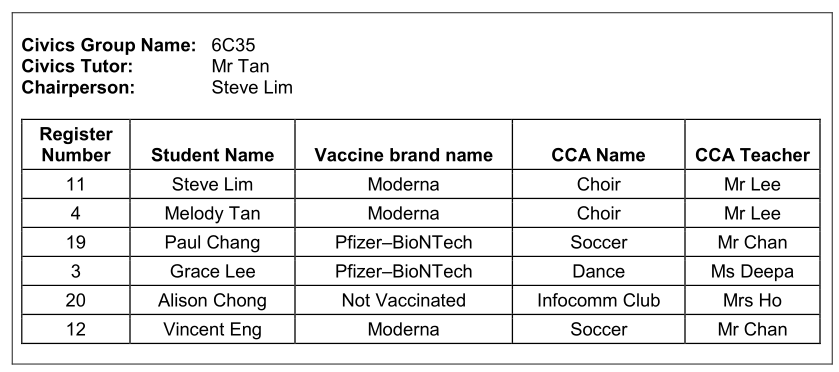
\includegraphics[width=0.5\paperwidth]{C:/Users/Admin/Desktop/Github/question_bank/static/img/9597-DHS-2021-P1-Q5}
\par\end{center}
\begin{enumerate}
\item Derive a set of tables to show the above data in first, second and
third normal form. \hfill{}{[}6{]}
\item Draw an ER diagram for a normalised database design. \hfill{} {[}2{]}
\item Using examples in the above context, explain the significance of the
following terms:
\begin{enumerate}
\item primary key \hfill{}{[}2{]}
\item foreign key \hfill{}{[}2{]}
\end{enumerate}
\item With reference to the above context, describe or suggest a scenario
where a NoSQL database would be more appropriate. \hfill{} {[}1{]}
\end{enumerate}